\section{Esercizio 21}

\textit{\textbf{Descrizione:}  Uno strumento di misura ha una accuratezza di $10^{-6}$ (in opportune unit\'a di misura). I dati misurati nelle posizioni $x_i$ sono dati da $y_i$, come descritto dalla seguente tabella. Calcolare il grado minimo, ed i relativi coefficienti, del polinomio che meglio approssima i precedenti dati nel senso dei minimi quadrati con una adeguata accuratezza. Graficare convenientemente i risultati ottenuti.\\ \\
\begin{tabular}{|c|c|c|}	%	TABELLA DATI ESERCIZIO
	\hline
	i &$x_i$ &$y_i$\\ \hline
	0 &0.010 &1.003626 \\ \hline
	1 &0.098 &1.025686 \\ \hline
	2 &0.127 &1.029512 \\ \hline
	3 &0.278 &1.029130 \\ \hline
	4 &0.547 &0.994781 \\ \hline
	5 &0.632 &0.990156 \\ \hline
	6 &0.815 &1.016687 \\ \hline
	7 &0.906 &1.057382 \\ \hline
	8 &0.913 &1.061462 \\ \hline
	9 &0.958 &1.091263 \\ \hline
	10& 0.965& 1.096476\\ \hline
\end{tabular}}
\newline
\noindent\emph{Soluzione: }\newline
Dare risposta a questo quesito significa andare a risolvere il sistema $Va=y$ nel senso dei minimi quadrati. Per $n=0...10$ andiamo ad iterare il nostro procedimento, imponendo un criterio di arresto sulla norma del vettore residuo $||r-n|| \leq 10^{-6}$.
Dobbiamo creare la matrice rettangolare di Vandermonde relativa ai valori $x_i$ e scomporla nei suoi fattori $\emph{Q}\in R^{mxm}$ ed $\emph{R}\in R^{mxn}$ relativi alla sua fattorizzazione \emph{QR}. Dato che \emph{Q} \'e ortogonale e $R=(\frac{\hat{R}}{0})$ ovvero \'e formata da una matrice quadrata $\hat{R}\in R^{nxn}$ triangolare superiore e per il resto \'e composta da zeri, calcoliamo il vettore $g_1$ con la formula $g = Q^Ty$ e $g = (\frac{g_1}{g_2})$ con $g_1 \in R^{n}$ e $g_2 \in R^{m-n}$. Nel nostro caso, avremo $m = 11$. Risolviamo quindi il sistema lineare $\hat{R}a=g_1$ per trovare i coefficienti del polinomio di grado \emph{n}.\\
Per ottenere quanto specificato, \'e stato utilizzato il seguente \emph{script}, che fornisce anche la visualizzazione grafica della norma del vettore residuo:\\
\section*{Risoluzione del sistema ai minimi quadrati:}
\lstinputlisting{resources/21Sistema.m}\newpage
\noindent L'output ci indica che il polinomio ha grado 3 e che i suoi coefficienti sono i seguenti:\newline
a0 = + 0.999999854479502\\
a1 = + 0.375001162045807\\
a2 = - 1.250002941638535\\
a3 = + 1.000001891005298

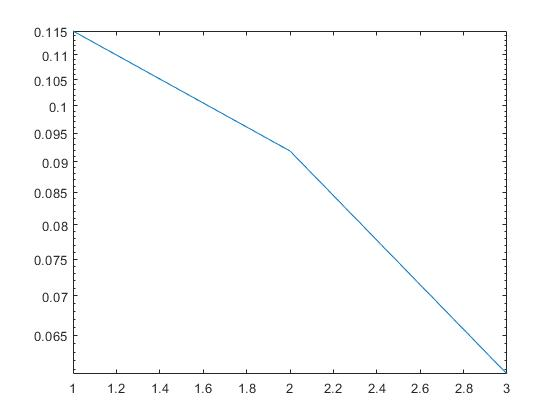
\includegraphics[width=1\linewidth]{img/21Norma.jpg}

